% This is "sig-alternate.tex" V2.0 May 2012
% This file should be compiled with V2.5 of "sig-alternate.cls" May 2012
%
% This example file demonstrates the use of the 'sig-alternate.cls'
% V2.5 LaTeX2e document class file. It is for those submitting
% articles to ACM Conference Proceedings WHO DO NOT WISH TO
% STRICTLY ADHERE TO THE SIGS (PUBS-BOARD-ENDORSED) STYLE.
% The 'sig-alternate.cls' file will produce a similar-looking,
% albeit, 'tighter' paper resulting in, invariably, fewer pages.
%
% ----------------------------------------------------------------------------------------------------------------
% This .tex file (and associated .cls V2.5) produces:
%       1) The Permission Statement
%       2) The Conference (location) Info information
%       3) The Copyright Line with ACM data
%       4) NO page numbers
%
% as against the acm_proc_article-sp.cls file which
% DOES NOT produce 1) thru' 3) above.
%
% Using 'sig-alternate.cls' you have control, however, from within
% the source .tex file, over both the CopyrightYear
% (defaulted to 200X) and the ACM Copyright Data
% (defaulted to X-XXXXX-XX-X/XX/XX).
% e.g.
% \CopyrightYear{2007} will cause 2007 to appear in the copyright line.
% \crdata{0-12345-67-8/90/12} will cause 0-12345-67-8/90/12 to appear in the copyright line.
%
% ---------------------------------------------------------------------------------------------------------------
% This .tex source is an example which *does* use
% the .bib file (from which the .bbl file % is produced).
% REMEMBER HOWEVER: After having produced the .bbl file,
% and prior to final submission, you *NEED* to 'insert'
% your .bbl file into your source .tex file so as to provide
% ONE 'self-contained' source file.
%
% ================= IF YOU HAVE QUESTIONS =======================
% Questions regarding the SIGS styles, SIGS policies and
% procedures, Conferences etc. should be sent to
% Adrienne Griscti (griscti@acm.org)
%
% Technical questions _only_ to
% Gerald Murray (murray@hq.acm.org)
% ===============================================================
%
% For tracking purposes - this is V2.0 - May 2012

\documentclass{sig-alternate}
\usepackage{graphicx}
\usepackage{epstopdf}
\usepackage{psfrag}
\usepackage{psfig}
\usepackage{cite}
\usepackage{enumerate}
\usepackage{amssymb}
\usepackage{bm}
\usepackage{algorithm} 
\usepackage{algorithmic} 
\usepackage{multirow} 
\usepackage{amsmath}
\usepackage{xcolor}
%\DeclareMathOperator*{argmin}{argmin} 
%\enewcommand{algorithmicrequire}{ extbf{Input:}} 
%\enewcommand{algorithmicensure}{ extbf{Output:}} 
\begin{document}
%
% --- Author Metadata here ---
\conferenceinfo{WOODSTOCK}{'97 El Paso, Texas USA}
%\CopyrightYear{2007} % Allows default copyright year (20XX) to be over-ridden - IF NEED BE.
%\crdata{0-12345-67-8/90/01}  % Allows default copyright data (0-89791-88-6/97/05) to be over-ridden - IF NEED BE.
% --- End of Author Metadata ---

\title{The ART of SQL Injection Vulnerabilities Discovery \titlenote{This research was supported by the Open Fund of the State Key Laboratory of Computer Science, Institute of Software, Chinese Academy of Sciences (Grant No. SYSKF1405).}}
%\subtitle{[Extended Abstract]
%\titlenote{A full version of this paper is available as
%\textit{Author's Guide to Preparing ACM SIG Proceedings Using
%\LaTeX$2_\epsilon$\ and BibTeX} at
%\texttt{www.acm.org/eaddress.htm}}
%
% You need the command \numberofauthors to handle the 'placement
% and alignment' of the authors beneath the title.
%
% For aesthetic reasons, we recommend 'three authors at a time'
% i.e. three 'name/affiliation blocks' be placed beneath the title.
%
% NOTE: You are NOT restricted in how many 'rows' of
% "name/affiliations" may appear. We just ask that you restrict
% the number of 'columns' to three.
%
% Because of the available 'opening page real-estate'
% we ask you to refrain from putting more than six authors
% (two rows with three columns) beneath the article title.
% More than six makes the first-page appear very cluttered indeed.
%
% Use the \alignauthor commands to handle the names
% and affiliations for an 'aesthetic maximum' of six authors.
% Add names, affiliations, addresses for
% the seventh etc. author(s) as the argument for the
% \additionalauthors command.
% These 'additional authors' will be output/set for you
% without further effort on your part as the last section in
% the body of your article BEFORE References or any Appendices.

\numberofauthors{6} %  in this sample file, there are a *total*
% of EIGHT authors. SIX appear on the 'first-page' (for formatting
% reasons) and the remaining two appear in the \additionalauthors section.
%
\author{
% You can go ahead and credit any number of authors here,
% e.g. one 'row of three' or two rows (consisting of one row of three
% and a second row of one, two or three).
%
% The command \alignauthor (no curly braces needed) should
% precede each author name, affiliation/snail-mail address and
% e-mail address. Additionally, tag each line of
% affiliation/address with \affaddr, and tag the
% e-mail address with \email.
% 
% 1st. author
\alignauthor
Chenghong Wang\\
%\titlenote{Dr.~Trovato insisted his name be first.}\\
       \affaddr{Harbin Engineering University}\\
%       \affaddr{144 Nantong Street}\\
       \affaddr{Harbin, China}\\
       \email{wangchenghong@hr-beu.edu.cn}
% 2nd. author
\alignauthor
Donghong Zhang\\
       \affaddr{Harbin Engineering University}\\
%       \affaddr{144 Nantong Street}\\
       \affaddr{Harbin, China}\\
       \email{zhangdonghong@hr-beu.edu.cn}
% 3rd. author
\alignauthor Jingyu Li\\
       \affaddr{Harbin Engineering University}\\
%       \affaddr{144 Nantong Street}\\
       \affaddr{Harbin, China}\\
       \email{lijingyu@hrbeu.edu.cn} 
\and  % use '\and' if you need 'another row' of author names
% 4th. author
\alignauthor Jing Zhao\titlenote{All correspondence should be forwarded to Dr. Jing Zhao}\\
       \affaddr{Harbin Engineering University}\\
       \affaddr{Harbin, China}\\
       \email{zhaoj@hrbeu.edu.cn} 
% 5th. author
\alignauthor Zhenyu Zhang\\
       \affaddr{Institute of Software}\\
       \affaddr{Chinese Academy of Sciences}\\
       \affaddr{Beijing 100190}\\
       \email{zhangzy@ios.ac.cn}
% 6th. author
\alignauthor Long Zhang\\
       \affaddr{Institute of Software}\\
       \affaddr{Chinese Academy of Sciences}\\
       \affaddr{Beijing 100190}\\
       \email{zlong@ios.ac.cn}
}
% There's nothing stopping you putting the seventh, eighth, etc.
% author on the opening page (as the 'third row') but we ask,
% for aesthetic reasons that you place these 'additional authors'
% in the \additional authors block, viz.
%\additionalauthors{Additional authors: John Smith (The Th{\o}rv{\"a}ld Group,
%email: {\texttt{jsmith@affiliation.org}}) and Julius P.~Kumquat
%(The Kumquat Consortium, email: {\texttt{jpkumquat@consortium.net}}).}
%\date{30 July 1999}
% Just remember to make sure that the TOTAL number of authors
% is the number that will appear on the first page PLUS the
% number that will appear in the \additionalauthors section.

\maketitle
\begin{abstract}
SQL injection(SQLi) is one of the  top risky vulnerabilities for web applications which may lead to significant security consequences such as authentication bypassing, privacy leakage, etc.. Therefore, discovering SQLi vulnerabilities is an important step for ensuring its quality. Effective testing techniques can ensure that applications are free from SQLi vulnerabilities before its been released and reduce related cost of performing manual analysis, monitoring or post deployment of other defensive mechanisms. However, due to the variety of SQLi attack types the generated test cases for discovering SQLi are scable and complex. Moreover, successful test cases which could discovery SQLi vulnerabilities consist only a small part of the whole test case space. Therefore, testing the SQLi vulnerabilities is a time consuming and inefficient task. Towards this problem we propose an effective SQLi testing approch based on Adaptive Random Testing(ART) method. We define the concept of test case distance and then present the computing method for test case distance by using TF-IDF algorithm. Then we apply the Fixed Size Candidate Set(FSCS) algorithm in SQLi test case selection with the help of test case distance metrics. We also conduct 6 experimental studies on our testing algorithm, where we tested the SQLi vulnerabilities in 4 open source benchmarks and 2 CMS applications. The experimental results indicate that our testing algorithm can reduce the redundant test cases by more than 50\% and significantly increases the testing effectiveness of SQLi vulnerabilities discovering techniques.
\end{abstract}
%A category including the fourth, optional field follows...
\category{D.2.5}{Software Engineering}{Testing and Debugging}
\terms{Security, Algorithms}

\keywords{SQL injection; adaptive random test; test case distance metrics; selection algorithm}

\section{Introduction}
Nowadays, database-driven web applications have been rapidly adopted in a wide range of areas including online stores, e-commerce, social network services, etc. However such popularity makes them more attractive to attackers. The number of reported web attacks is growing sharply\cite{web_security:report}. A recent web application attack report show us that, over a period of nine months, from August 1, 2013 to April 30, 2014 reveals an average increase of around 17\% in different types of web attacks. In addition, the report also found that web attacks have became more sophisticated and gotten dramatically longer in length.(44\% longer than they were in previous reports). Web applications are suffering more than 26 attacks in one minute\cite{web_security:report2}. Other security report indicate that at least 8\% of the web services which belong to some technology companies like Microsoft and Google contains different types of security vulnerabilities\cite{dsn09:scanner}.

Within the Web based vulnerabilities, SQLi vulnerabilities has been labeled as top risky vulnerabilities by {Open Web Application Security\footnote{http://www.programmableweb.com,}}. SQLi refers to a class of code-injection attacks in which data provided by the user is included in a SQL query in such a way that part of the user's input is treated as SQL code\cite{ase05:amneisa}. This type of vulnerability is ultimately caused by insufficient validation of user-input\cite{ase05:amneisa, halfond07:detection, halfond06:classification}. By exploiting such vulnerabilities, attackers can submit malicious requests which contains sophisticated SQL queries to remote database-driven web applications. As a result, attackers will capture the privilege of accessing the underlying database arbitrarily. Attackers can even take control of and corrupt the system that hosts the Web applications by elaborately designing the injected SQL codes. During the past few years, SQLi vulnerabilities have already became the top 1 threat for database-driven web applications, and SQL injection attacks have also become the most popular web attack. 

Although the cause for SQLi is quite simple and the mechanisms of SQLi are well-understood, the SQLi vulnerabilities still increase. They persist because of a lack of effective techniques for discovering and preventing them. Previous approaches to detecting SQLi  vulnerabilities and preventing exploits include static analysis\cite{su06essence, livshits05finding, fu2007static}, user input filtering\cite{leblanc2002writing}, defensive programming\cite{cook2005safe}, runtime monitoring\cite{buehrer2005using, halfond2006using, pietraszek2006defending, su2006essence}, combining static analysis and runtime monitoring\cite{ase05:amneisa}, source code fixing\cite{thomas2007using}, application level intrusion detecting\cite{lin2007automatic}, SQL key words randomization\cite{boyd2004sqlrand}, testing techniques\cite{shahriar2008music, appelt2014automated, kieyzun2009automatic}, etc.. Among these previous researches, it is well accepted that security testing method is the most effective way towards discovering SQLi vulnerabilities. Security testing against SQLi vulnerabilities could significantly reduce the related costs of static analysis, monitoring or deploy application level defensive mechanisms, which are acknowledged time consuming and inefficient tasks. On the other hand, security test could guarantee the web applications free from SQLi vulnerabilities before they go into services. It is much easier to repair the applications before the applications' service lifecycle than during such period. However, very few works address the issues of testing techniques towards SQLi vulnerabilities, as SQLi testing suffers from three well-known problems. The problems for SQLi testing could be conclude as follows:
\begin{enumerate}[a)]
\item \emph{Scalability of Test Case Space}

The difficulty for researchers to address the full scope of the SQLi vulnerabilities is that there are many types of SQLI attacks and countless variations on these basic types. As a result, the test case space should be designed as large as possible. Otherwise some effective attack vectors which could reveal the potential SQLi vulnerabilities of testing applications may be missed.( i.e. Functions and keywords filtering prevents web applications from being attacked by using a functions and keywords black list. If an attackers submits an injection code containing a keyword or SQL function in the black list, the injection will be unsuccessful. Although the technique is very strict and perform in real world, applications with such security mechanism may also vulnerable to SQLi attacks. Attacks can evade inspection by using case changing, character encoding or inline comment methods.) Therefore, it is important to design enough test cases for testing. Equally the scale of test case space increase to a great level.
\item \emph{Sparse Distribution of Effective Test Cases}

Though the test case space is very large, the effective test cases which could flag SQLi vulnerabilities distributed sparsely. In our previous works, we found that the effective test cases for SQLi discovery consist only 2\% of the total test case pool. Such small proportion makes the searching task for effective test cases more difficult than normal testing tasks. And the performing of rest 98\% can be regard as redundant works which may limit the testing effectiveness. 
\item \emph{Large Expense for Executing SQLi Test Cases}

The performing costs for SQLi vulnerabilities discovery are also very high. The judgement of test cases execution results could be a complex work. Some researchers have proposed some automatic mechanism for testing result checking and judging\cite{appelt2014automated, damele2012sqlmap, riancho2011w3af}. However, in some cases, it also requires some professional testers to complete the checking and judging tasks manually. i.e. In some web applications the injectable parameters appear in some particular sections like HTTP Head Referer (CVE-2011-3340\footnote{http://cve.mitre.org/cgi-bin/cvename.cgi?name=CVE-2011-3340}, CVE-2008-0850\footnote{http://cve.mitre.org/cgi-bin/cvename.cgi?name=CVE-2008-0850}, CVE-2007-1061\footnote{http://cve.mitre.org/cgi-bin/cvename.cgi?name=CVE-2007-1061}) section. In this cases, the most accurate and effective way to check or judge the testing is to check by testing engineers. Testing engineer have to check every test cases results during the testing period. 
\end{enumerate}

According to all the aforementioned problems of SQLi testing techniques, we know that SQLi testing is indeed a timing consuming and complex task compared to normal software testing. Moreover the high level of testing redundancy for SQLi vulnerabilities discovering even amplify the testing ineffectiveness and complexity. How to reduce the verbosity of test cases have became an important problem for improving SQLi testing effectiveness. To address this problem, we propose a test case selection algorithm for SQLi vulnerabilities discovering in this paper based on Adaptive Random Testing(ART) method. Through various empirical observations showing that many successful test cases are very similar between each others (i.e. Some are encoded by the same encoding method or attached with similar prefix.). More specifically, the successful test cases which could discovery SQLi have a high degree of similarity. As a result successful test cases distributed together to form clusters in total test cases domain. 

Due to this distribution of successful test cases, ART is supposed to be the best choice to improve the effectiveness of test case selection tasks. In our work, the approach started from test cases distance metrics quantification, in this part we apply the TF-IDF algorithm to compute the test cases distance due to the previous observation consequences of the successful SQLi test cases distribution. Then we apply a well performed Adaptive Random Testing method called Fixed Size Candidate Set(FSCS) method to select test cases with the help of test cases distance metrics. Through FSCS algorithm, the test case selected to execute should be the most distinct (the farthest) one compared to the previous one. It is because that regions of the unsuccessful test cases domain will also be contiguous. Thus, given a set of previously executed test cases that have not revealed any failures, new test cases located away from these old ones are more likely to reveal failures. 

We have also evaluated our test cases selection algorithm by comparing the discovering effectiveness of some reported vulnerabilities(reported on National Vulnerability Database) between testing approach with and without FSCS-ART algorithm. The statistic used to compare the methods was the average number of tests required to detect the first successful test case, which is commonly known as the F-measure\cite{chen2005adaptive}. In most cases, the F-measure of FSCS-ART was 30-50\% lower than that of testing approach without ART selection algorithm. Experimental result indicate that our selection can significantly reduce the SQLi testing redundancy and increase the SQLi vulnerabilities discovering effectiveness.

The main contributions of this work are:
\begin{itemize}
\item The presentation of a new technique to test SQLi vulnerabilities that based on adaptive random method.
\item The observation and analysis of effective test case distribution for dectecting SQLi vulnerabilities which shows that successful test case tend to be clustered together. 
\item The presentation of test case distance metrics based on string similarity metrics.
\item An experimental evaluation of the technique that shows the effectiveness
and the efficiency of this technique.
\end{itemize}

The remainder of this paper is organised as follows: Section 2 and Section 3 provides a background on SQLi vulnerabilities and reviews related work. Section 4 is the introduction of Adaptive Random Testing and discussion of successful SQLi test case distribution. Section 5 presents our proposed security testing approach. Section 6 presents the evaluation together with a discussion of results and threats to validity. Finally, Section 7 concludes the work.



\section{Background of SQLi}
\subsection{Injection Mechanisms}
\subsection{Example of SQL injections}
\section{Related Works}
\subsection{SQLi Prevention}
\subsection{Adaptive Random Testing}
Adaptive Random Testing (ART) is an effective improvement of Random Testing (RT). It is based on the observation effective test cases for testing target program tend to be clustered together. ART, therefore, proposes to have randomly selected test cases being more evenly spread throughout the test case domain by employing the location information of the successful test cases.\cite{39239038}

\section{Test Case Distributions}
Essentially, the testing process can be viewed as taking samples
from the set of all SQLi attack payloads(known as the test case space) to the web application under test, executing the samples one by one, and determining whether the malicious inouts been filtered by input validation mechanisms of testing application. If the inputs get through, a payload bypassing is revealed. The presence of a bypassing implies the existence of a SQLi vulnerability. A tester seeks to select test data 
with a view to minimising the cost for detecting SQLi vulnerabilities. 
To help the tester in this task, it is natural to firstly consider how
effective test cases distribute in total test cases space.

To present our work clearly, let us first define a few terms. Suppose $\mathit{T}$ = \{$t_{1}$, $t_{2}$, $t_{3}$, ... , $t_{n}$ \} is a SQLi test case space for some specific web application program (denoted by $P$) with $n$ test cases. For each test case $t_{i}$ in $T$ is a type of specific string which could be injeted into web applications through input functions and flag SQLi attacks, we also call these strings SQLi attack payloads. Within test case space $T$ we define $S$ = \{$s_{1}$, $s_{2}$, $s_{3}$, ... , $s_{k}$ \} to be the effective test cases set with total $k$ test cases, where every test case $s_{i}$ in $S$ can successfully flag SQLi vulnerabilities in application $P$. On the other hand $F$ = \{$f_{1}$, $f_{2}$, $f_{3}$, ... , $f_{d}$ \} are defined as ineffective test cases set or redundant test cases set such that $ F, S\subseteq T$ and $F \cap S = \varnothing$.
The size number of total test case space, effective test case space and redundant test case space are denoted by $n, k, d$ respectively, where $n = k + d$.

In our recent works, we have tested 29 reported SQLi vulnerabilities (Reported on NVD) by using the test cases (SQLi attack payloads) from real world. After that we have two observations from our testing. First, the test cases space collected for dectecting SQLi vulnerabilities is very huge, in other word the $n$ is very large. However, the effective test cases consist only a small part of the test cases space, the successful ratio $k / n$ is always below 2 percent. Second, effective SQLi test cases which could detect some specific SQLi vulnerability are always have the similar string format or constructure. 

Let's take the CVE-2010-0425~(a reported SQLi vulnerability) as an example. Table I is the effective test cases we collected in our testing, it shows that the effective test cases for detecting CVE-2010-0425 are all similar to each others. All successful test cases are tautology attack payloads and the injection type are all the time based blind SQL injection mode (they contain the same terms like waitfor, delay, which are the key words for time based blind SQLi). To improve that the effective test cases share high similarity between each others, we select one effective test case $s_{j}$ and then compute the string similarity between $s_{j}$ and other test cases used for dectecting CVE-2010-0425.

\begin{table}
\centering
\caption{Successful Test Cases for CVE2010-0415}
\begin{tabular}{|c|c|l|} \hline
No.&Sucessful Test Case\\ \hline
1 & ; or 1 = 1 waitfor delay '0: 0: TIME --\\ \hline
2 & ); or 1 = 1 waitfor delay '0: 0: TIME --\\ \hline
3 & '; or 1 = 1 waitfor delay '0: 0: TIME --\\ \hline
4 & "; or 1 = 1 waitfor delay '0: 0: TIME --\\ \hline
5 & '); or 1 = 1 waitfor delay '0: 0: TIME --\\ \hline
6 & "); or 1 = 1 waitfor delay '0: 0: TIME --\\ \hline
7 & )); or 1 = 1 waitfor delay '0: 0: TIME --\\ \hline
8 & ')); or 1 = 1 waitfor delay '0: 0: TIME --\\ \hline
... & ...\\
\hline\end{tabular}
\end{table}

From the details we observed, we can conclude that, effective SQLi test cases for testing target tend to be clustered together within whole test case domain, in other word if $s_{j}$ is an effective test cases twords some specific SQLi vulnerability, the test cases close to $s_{j}$ (similar with $s_{j}$ in string format) will more likely to reveal such vulnerability.

\section{The ART of SQLi Discovery}
Clustering distribution of effective test cases for detecting SQLi are indeed common. Therefore, given a set of previously executed
test cases that have not revealed SQLi vulnerabilities, new test cases
located away from(string format distinct from) these old ones are more likely to reveal vulnerabilities-in other words, test cases should be more evenly spread
throughout the total test case space. According to this intuition, Adaptive
Random Testing (ART) method was applied to improve the effectiveness of SQLi discovering technique.
\subsection{Test Case Similarity Metrics}
From our previous observation of effective SQLi test cases, we found that they, effective SQLi test cases, tend to be clustered together from the string structure point of view. Thus, we define the test case distance metrics based on the string similarity and propose TF-ITSF(Term Frequency-Inverse Testcase Space Frequency) method to quantify test case similarity.\\ 

{\bf Definition 1 [Test Case Term Space]}~Each SQLi test case is a type of string, the elements consist of such string are called test cases terms. Suppose $T$ is the test case space for application $P$. Then, $TS = \{tm_{1},tm_{2},...,tm_{t}\}$ is the test case term space of $T$, denote the set of all distinct terms appear in whole test case space. The element terms in SQLi test cases area not the same terms in documents, they are more complicated. Table 2 provides a summary of the terms in SQLi test cases.\\








{\bf Definition 2 [Test Case Feature Vector]}~Suppose $T = \{t_{1}, t_{2}, t_{3},...,  t_{n}\}$ is the test case space of testing application $P$, and $TS = \{tm_{1}, tm_{2}, tm_{3},..., tm_{k}\}$ is the term space, denote $k$ distinct terms in total test case space. And for each test case $t_{j}$, the feature vector of $t_{j}$ is denote as  ${\bf  d_{j}} = [{w_{1,j}, w_{2,j}, w_{3,j} ... , w_{k,j}]^\mathrm{T}}$. Each dimension is called the (term) weight corresponds to a separate term in $TS$, where 

\begin{equation}w_{i,j} = \frac { \log{(TF_{i,j} + 1.0)} \times \log \frac{|T|}{|\{t^{'} : tm_i \in t^{'}\}|} }
{\sqrt{ \sum_{i=1}^{k} \lbrack \log{(TF_{i,j} + 1.0)} \times \log \frac{|T|}{|\{t^{'} : tm_i \in t^{'}\}|}\rbrack ^{2} }}
\end{equation}


\begin{itemize}
\item $TF_{i,j}$ is the term frequency of term $tm_{i}$ in test case $t_{j}$.
\item $|T|$ is total number of test cases , and ${|\{t^{'} : tm_i \in t^{'}\}|}$, is number of test cases containing term $tm_{i}$.
\end{itemize} 

Usually, ${\bf  d_{j}}$ is a column vector with high level dimensions, thus such feature vector will bring lot of costs in computing procedures. Here we apply Principal Component Analysis (PCA) method to reduce ${\bf  d_{j}}$.\\

{\bf Definition 3 [Test Case Distance Metrics]}~Suppose two test case $t_{i}$ and $t_{q}$, their feature vectors are\\ ${\bf d_{j}} = [w_{1,j}, w_{2,j}, w_{3,j},...,w_{k,j}]$, ${\bf d_{q}} = [w_{1,q}, w_{2,q}, w_{3,q},...,w_{k,q}]$. We define the distance between test case $t_{i}$ and $t_{q}$ by using Cosine Distance( or Cosine Similarity ) measurement. Such distance is represented as follows:

\begin{equation}dis(t_{j}, t_{q}) = \frac{  {\bf d_{j}} \cdot {\bf d_{q} } }{ || {\bf d_{j} } || ~||  {\bf d_{q}} || } = \frac{ \sum_{i=1}^{k} w_{i,j}\cdot w_{i,q} }{\sqrt{  \sum_{i=1}^{k} w_{i,j}^{2} } \cdot \sqrt{ \sum_{i=1}^{k} w_{i,q}^{2}  }  }\end{equation}

In definition 2 , it is obviously that $\forall ~t_{i}~ in ~T$ , the (term) weight in feature vector $\bf d_{i}$ are all belongs to $\mathbb{R}$. Therefore, the outcome of Equation (2), test cases distance (similarity), is neatly bounded in $\lbrack ~0, 1 ~\rbrack$. The resulting distance (similarity) ranges from 0 indicating orthogonality (decorrelation), to 1 meaning exactly the same, and in-between values indicating intermediate similarity.




\subsection{Candidate Test Case Selection Algorithm}
In this paper,  we use the first ART method proposed, Fixed Size Candidate Set (FSCS)[**] algorithm to select candidate test cases. During the test case selection procedure, we apply adaptive random testing method in candidate test case selection algorithm to realize the aforementioned purpose. In our process, the selection algorithm makes use of two sets of test cases, named executed set and candidate set which. Suppose $E = \{e_{1}, e_{2}, e_{3}, ..., e_{f}\}$ is the executed set, and $C= \{c_{1}, c_{2}, c_{3}, ..., c_{g}\}$ be the candidate set such that $E \cap C = \emptyset$.  


 $E$ is the set of distinct test cases that have already been selected and executed but without revealing any SQLi vulnerability while the $C$ is a set of test cases that are randomly selected from $T$. The executed set is initially empty and the first test case is randomly chosen from the test case space. The executed set is then incrementally updated with the selected element $c_{h}$, ( $c_{h} \in C$ ) until a SQLi vulnerability is revealed. The selected element $c_{h}$ should satisfy the following condition:
For all $ j \in \{1, 2, 3, ..., g\} $, $$\min_{i=1}^{f} dis(c_{h}, e_{i}) \geq \min_{i=1}^{f} dis(c_{j}, e_{i}) $$
where $dis$ is defined in Definition 3. Specific algorithm of FSCS-ART is described in Algorithm \ref{alg:Framwork}.

\renewcommand{\algorithmicrequire}{ \textbf{Input:}} %Use Input in the format of Algorithm
\renewcommand{\algorithmicensure}{ \textbf{Output:}} %UseOutput in the format of Algorithm
\begin{algorithm}[htb] 
\caption{ ~Fixed Size Candidate Set - ART } 
\label{alg:Framwork} 
\begin{algorithmic}[1] %??1 ??????????
\REQUIRE ~~\\ %????????Input
The set of test case space for application $P$, $T$;\\
The size of candidate test case set, $\kappa$;\bigskip\\
%\ENSURE ~~\\ %??????Output
%Ensemble of classifiers on the current batch, $E_n$;\bigskip\\
\STATE $E$ = \{\}
\STATE $C$ = \{\}
\label{ code:fram:extract }%?????????????????????
\STATE Training ensemble of classifiers $E$ on $T_n \cup P_n$, with help of data in former batches; 
\label{code:fram:trainbase}
\STATE $E_n=E_{n-1}\cup E$; 
\label{code:fram:add}
\STATE Classifying samples in $U_n-T_n$ by $E_n$; 
\label{code:fram:classify}
\STATE Deleting some weak classifiers in $E_n$ so as to keep the capacity of $E_n$; 
\label{code:fram:select}
\RETURN $E_n$; %??????
\end{algorithmic}
\end{algorithm}


\section{Experiments}
\subsection{Experiment Setup}
\subsection{Scenarios}
\subsection{Result \& Analysis}

%\section{Related Works}


\section{Conlusion}

\bibliographystyle{abbrv}
\bibliography{sqli} 

\section{The {\secit Body} of The Paper}
Typically, the body of a paper is organized
into a hierarchical structure, with numbered or unnumbered
headings for sections, subsections, sub-subsections, and even
smaller sections.  The command \texttt{{\char'134}section} that
precedes this paragraph is part of such a
hierarchy.\footnote{This is the second footnote.  It
starts a series of three footnotes that add nothing
informational, but just give an idea of how footnotes work
and look. It is a wordy one, just so you see
how a longish one plays out.} \LaTeX\ handles the numbering
and placement of these headings for you, when you use
the appropriate heading commands around the titles
of the headings.  If you want a sub-subsection or
smaller part to be unnumbered in your output, simply append an
asterisk to the command name.  Examples of both
numbered and unnumbered headings will appear throughout the
balance of this sample document.

Because the entire article is contained in
the \textbf{document} environment, you can indicate the
start of a new paragraph with a blank line in your
input file; that is why this sentence forms a separate paragraph.

\subsection{Type Changes and {\subsecit Special} Characters}
We have already seen several typeface changes in this sample.  You
can indicate italicized words or phrases in your text with
the command \texttt{{\char'134}textit}; emboldening with the
command \texttt{{\char'134}textbf}
and typewriter-style (for instance, for computer code) with
\texttt{{\char'134}texttt}.  But remember, you do not
have to indicate typestyle changes when such changes are
part of the \textit{structural} elements of your
article; for instance, the heading of this subsection will
be in a sans serif\footnote{A third footnote, here.
Let's make this a rather short one to
see how it looks.} typeface, but that is handled by the
document class file. Take care with the use
of\footnote{A fourth, and last, footnote.}
the curly braces in typeface changes; they mark
the beginning and end of
the text that is to be in the different typeface.

You can use whatever symbols, accented characters, or
non-English characters you need anywhere in your document;
you can find a complete list of what is
available in the \textit{\LaTeX\
User's Guide}\cite{Lamport:LaTeX}.

\subsection{Math Equations}
You may want to display math equations in three distinct styles:
inline, numbered or non-numbered display.  Each of
the three are discussed in the next sections.

\subsubsection{Inline (In-text) Equations}
A formula that appears in the running text is called an
inline or in-text formula.  It is produced by the
\textbf{math} environment, which can be
invoked with the usual \texttt{{\char'134}begin. . .{\char'134}end}
construction or with the short form \texttt{\$. . .\$}. You
can use any of the symbols and structures,
from $\alpha$ to $\omega$, available in
\LaTeX\cite{Lamport:LaTeX}; this section will simply show a
few examples of in-text equations in context. Notice how
this equation: \begin{math}\lim_{n\rightarrow \infty}x=0\end{math},
set here in in-line math style, looks slightly different when
set in display style.  (See next section).

\subsubsection{Display Equations}
A numbered display equation -- one set off by vertical space
from the text and centered horizontally -- is produced
by the \textbf{equation} environment. An unnumbered display
equation is produced by the \textbf{displaymath} environment.

Again, in either environment, you can use any of the symbols
and structures available in \LaTeX; this section will just
give a couple of examples of display equations in context.
First, consider the equation, shown as an inline equation above:
\begin{equation}\lim_{n\rightarrow \infty}x=0\end{equation}
Notice how it is formatted somewhat differently in
the \textbf{displaymath}
environment.  Now, we'll enter an unnumbered equation:
\begin{displaymath}\sum_{i=0}^{\infty} x + 1\end{displaymath}
and follow it with another numbered equation:
\begin{equation}\sum_{i=0}^{\infty}x_i=\int_{0}^{\pi+2} f\end{equation}
just to demonstrate \LaTeX's able handling of numbering.

\subsection{Citations}
Citations to articles \cite{bowman:reasoning,
clark:pct, braams:babel, herlihy:methodology},
conference proceedings \cite{clark:pct} or
books \cite{salas:calculus, Lamport:LaTeX} listed
in the Bibliography section of your
article will occur throughout the text of your article.
You should use BibTeX to automatically produce this bibliography;
you simply need to insert one of several citation commands with
a key of the item cited in the proper location in
the \texttt{.tex} file \cite{Lamport:LaTeX}.
The key is a short reference you invent to uniquely
identify each work; in this sample document, the key is
the first author's surname and a
word from the title.  This identifying key is included
with each item in the \texttt{.bib} file for your article.

The details of the construction of the \texttt{.bib} file
are beyond the scope of this sample document, but more
information can be found in the \textit{Author's Guide},
and exhaustive details in the \textit{\LaTeX\ User's
Guide}\cite{Lamport:LaTeX}.

This article shows only the plainest form
of the citation command, using \texttt{{\char'134}cite}.
This is what is stipulated in the SIGS style specifications.
No other citation format is endorsed or supported.

\subsection{Tables}
Because tables cannot be split across pages, the best
placement for them is typically the top of the page
nearest their initial cite.  To
ensure this proper ``floating'' placement of tables, use the
environment \textbf{table} to enclose the table's contents and
the table caption.  The contents of the table itself must go
in the \textbf{tabular} environment, to
be aligned properly in rows and columns, with the desired
horizontal and vertical rules.  Again, detailed instructions
on \textbf{tabular} material
is found in the \textit{\LaTeX\ User's Guide}.

Immediately following this sentence is the point at which
Table 1 is included in the input file; compare the
placement of the table here with the table in the printed
dvi output of this document.

\begin{table}
\centering
\caption{Frequency of Special Characters}
\begin{tabular}{|c|c|l|} \hline
Non-English or Math&Frequency&Comments\\ \hline
\O & 1 in 1,000& For Swedish names\\ \hline
$\pi$ & 1 in 5& Common in math\\ \hline
\$ & 4 in 5 & Used in business\\ \hline
$\Psi^2_1$ & 1 in 40,000& Unexplained usage\\
\hline\end{tabular}
\end{table}

To set a wider table, which takes up the whole width of
the page's live area, use the environment
\textbf{table*} to enclose the table's contents and
the table caption.  As with a single-column table, this wide
table will ``float" to a location deemed more desirable.
Immediately following this sentence is the point at which
Table 2 is included in the input file; again, it is
instructive to compare the placement of the
table here with the table in the printed dvi
output of this document.


\begin{table*}
\centering
\caption{Some Typical Commands}
\begin{tabular}{|c|c|l|} \hline
Command&A Number&Comments\\ \hline
\texttt{{\char'134}alignauthor} & 100& Author alignment\\ \hline
\texttt{{\char'134}numberofauthors}& 200& Author enumeration\\ \hline
\texttt{{\char'134}table}& 300 & For tables\\ \hline
\texttt{{\char'134}table*}& 400& For wider tables\\ \hline\end{tabular}
\end{table*}
% end the environment with {table*}, NOTE not {table}!

\subsection{Figures}
Like tables, figures cannot be split across pages; the
best placement for them
is typically the top or the bottom of the page nearest
their initial cite.  To ensure this proper ``floating'' placement
of figures, use the environment
\textbf{figure} to enclose the figure and its caption.

This sample document contains examples of \textbf{.eps}
and \textbf{.ps} files to be displayable with \LaTeX.  More
details on each of these is found in the \textit{Author's Guide}.

\begin{figure}
\centering
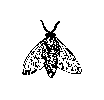
\epsfig{file=fly.eps}
\caption{A sample black and white graphic (.eps format).}
\end{figure}

\begin{figure}
\centering
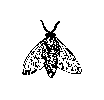
\epsfig{file=fly.eps, height=1in, width=1in}
\caption{A sample black and white graphic (.eps format)
that has been resized with the \texttt{epsfig} command.}
\end{figure}


As was the case with tables, you may want a figure
that spans two columns.  To do this, and still to
ensure proper ``floating'' placement of tables, use the environment
\textbf{figure*} to enclose the figure and its caption.
and don't forget to end the environment with
{figure*}, not {figure}!

\begin{figure*}
\centering
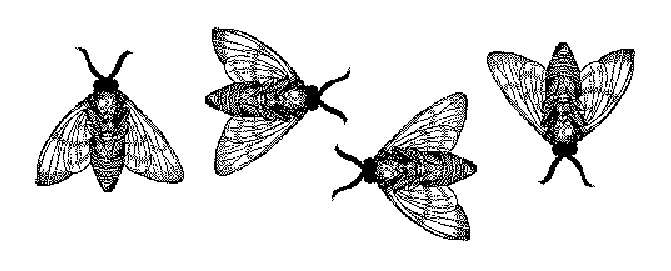
\epsfig{file=flies.eps}
\caption{A sample black and white graphic (.eps format)
that needs to span two columns of text.}
\end{figure*}

Note that either {\textbf{.ps}} or {\textbf{.eps}} formats are
used; use
the \texttt{{\char'134}epsfig} or \texttt{{\char'134}psfig}
commands as appropriate for the different file types.

\begin{figure}
\centering
\psfig{file=rosette.ps, height=1in, width=1in,}
\caption{A sample black and white graphic (.ps format) that has
been resized with the \texttt{psfig} command.}
\vskip -6pt
\end{figure}

\subsection{Theorem-like Constructs}
Other common constructs that may occur in your article are
the forms for logical constructs like theorems, axioms,
corollaries and proofs.  There are
two forms, one produced by the
command \texttt{{\char'134}newtheorem} and the
other by the command \texttt{{\char'134}newdef}; perhaps
the clearest and easiest way to distinguish them is
to compare the two in the output of this sample document:

This uses the \textbf{theorem} environment, created by
the\linebreak\texttt{{\char'134}newtheorem} command:
\newtheorem{theorem}{Theorem}
\begin{theorem}
Let $f$ be continuous on $[a,b]$.  If $G$ is
an antiderivative for $f$ on $[a,b]$, then
\begin{displaymath}\int^b_af(t)dt = G(b) - G(a).\end{displaymath}
\end{theorem}

The other uses the \textbf{definition} environment, created
by the \texttt{{\char'134}newdef} command:
\newdef{definition}{Definition}
\begin{definition}
If $z$ is irrational, then by $e^z$ we mean the
unique number which has
logarithm $z$: \begin{displaymath}{\log e^z = z}\end{displaymath}
\end{definition}

Two lists of constructs that use one of these
forms is given in the
\textit{Author's  Guidelines}.
 
There is one other similar construct environment, which is
already set up
for you; i.e. you must \textit{not} use
a \texttt{{\char'134}newdef} command to
create it: the \textbf{proof} environment.  Here
is a example of its use:
\begin{proof}
Suppose on the contrary there exists a real number $L$ such that
\begin{displaymath}
\lim_{x\rightarrow\infty} \frac{f(x)}{g(x)} = L.
\end{displaymath}
Then
\begin{displaymath}
l=\lim_{x\rightarrow c} f(x)
= \lim_{x\rightarrow c}
\left[ g{x} \cdot \frac{f(x)}{g(x)} \right ]
= \lim_{x\rightarrow c} g(x) \cdot \lim_{x\rightarrow c}
\frac{f(x)}{g(x)} = 0\cdot L = 0,
\end{displaymath}
which contradicts our assumption that $l\neq 0$.
\end{proof}

Complete rules about using these environments and using the
two different creation commands are in the
\textit{Author's Guide}; please consult it for more
detailed instructions.  If you need to use another construct,
not listed therein, which you want to have the same
formatting as the Theorem
or the Definition\cite{salas:calculus} shown above,
use the \texttt{{\char'134}newtheorem} or the
\texttt{{\char'134}newdef} command,
respectively, to create it.

\subsection*{A {\secit Caveat} for the \TeX\ Expert}
Because you have just been given permission to
use the \texttt{{\char'134}newdef} command to create a
new form, you might think you can
use \TeX's \texttt{{\char'134}def} to create a
new command: \textit{Please refrain from doing this!}
Remember that your \LaTeX\ source code is primarily intended
to create camera-ready copy, but may be converted
to other forms -- e.g. HTML. If you inadvertently omit
some or all of the \texttt{{\char'134}def}s recompilation will
be, to say the least, problematic.

\section{Conclusions}
This paragraph will end the body of this sample document.
Remember that you might still have Acknowledgments or
Appendices; brief samples of these
follow.  There is still the Bibliography to deal with; and
we will make a disclaimer about that here: with the exception
of the reference to the \LaTeX\ book, the citations in
this paper are to articles which have nothing to
do with the present subject and are used as
examples only.
%\end{document}  % This is where a 'short' article might terminate

%ACKNOWLEDGMENTS are optional
\section{Acknowledgments}
This section is optional; it is a location for you
to acknowledge grants, funding, editing assistance and
what have you.  In the present case, for example, the
authors would like to thank Gerald Murray of ACM for
his help in codifying this \textit{Author's Guide}
and the \textbf{.cls} and \textbf{.tex} files that it describes.

%
% The following two commands are all you need in the
% initial runs of your .tex file to
% produce the bibliography for the citations in your paper.
%\bibliographystyle{abbrv}
%\bibliography{sigproc}  % sigproc.bib is the name of the Bibliography in this case
% You must have a proper ".bib" file
%  and remember to run:
% latex bibtex latex latex
% to resolve all references
%
% ACM needs 'a single self-contained file'!
%
%APPENDICES are optional
%\balancecolumns
\appendix
%Appendix A
\section{Headings in Appendices}
The rules about hierarchical headings discussed above for
the body of the article are different in the appendices.
In the \textbf{appendix} environment, the command
\textbf{section} is used to
indicate the start of each Appendix, with alphabetic order
designation (i.e. the first is A, the second B, etc.) and
a title (if you include one).  So, if you need
hierarchical structure
\textit{within} an Appendix, start with \textbf{subsection} as the
highest level. Here is an outline of the body of this
document in Appendix-appropriate form:
\subsection{Introduction}
\subsection{The Body of the Paper}
\subsubsection{Type Changes and  Special Characters}
\subsubsection{Math Equations}
\paragraph{Inline (In-text) Equations}
\paragraph{Display Equations}
\subsubsection{Citations}
\subsubsection{Tables}
\subsubsection{Figures}
\subsubsection{Theorem-like Constructs}
\subsubsection*{A Caveat for the \TeX\ Expert}
\subsection{Conclusions}
\subsection{Acknowledgments}
\subsection{Additional Authors}
This section is inserted by \LaTeX; you do not insert it.
You just add the names and information in the
\texttt{{\char'134}additionalauthors} command at the start
of the document.
\subsection{References}
Generated by bibtex from your ~.bib file.  Run latex,
then bibtex, then latex twice (to resolve references)
to create the ~.bbl file.  Insert that ~.bbl file into
the .tex source file and comment out
the command \texttt{{\char'134}thebibliography}.
% This next section command marks the start of
% Appendix B, and does not continue the present hierarchy
\section{More Help for the Hardy}
The sig-alternate.cls file itself is chock-full of succinct
and helpful comments.  If you consider yourself a moderately
experienced to expert user of \LaTeX, you may find reading
it useful but please remember not to change it.
%\balancecolumns % GM June 2007
% That's all folks!
\end{document}
